%!TEX root = Slic3r-Manual.tex

\section{Fighting Ooze} % (fold)
\label{sec:fighting_ooze}
\index{ooze}
\index{retraction}

Unless the material being extruded has a very high viscosity it will ooze from the nozzle in between extrusions.  There are several settings in Slic3r to which can help to remedy this.

The retraction settings, found in the \texttt{Printer} tab, tell the printer to pull back the filament between extrusion moves.  This can alleviate the pressure in the nozzle, thus reducing ooze.  After the subsequent travel move the retraction is reversed to prepare the extruder for the next extrusion.

\begin{figure}[H]
\centering
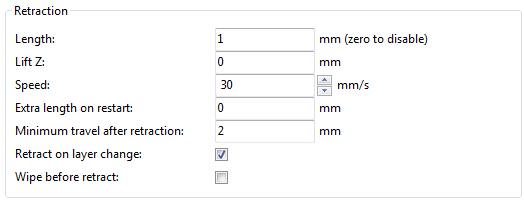
\includegraphics[keepaspectratio=true,width=1.0\textwidth]{expertmode/retraction_settings.png}
\caption{Retraction settings.}
\label{fig:retraction_settings}
\end{figure}
\index{Printer Settings!Extruder!Retraction!Length}
\index{Printer Settings!Extruder!Retraction!Lift Z}
\index{Printer Settings!Extruder!Retraction!Speed}
\index{Printer Settings!Extruder!Retraction!Extra length on restart}
\index{Printer Settings!Extruder!Retraction!Minimum travel after retraction}
\index{Printer Settings!Extruder!Retraction!Retract on layer change}
\index{Printer Settings!Extruder!Retraction!Wipe before retract}

\begin{itemize}
    \item \texttt{Length} - The number of millimeters to retract.  Note that the measurement is taken from the raw filament entering the extruder.  A value of between 1 and 2mm is usually recommended. Bowden extruders may need up to 4 or 5mm due to the hysteresis introduced by the tube.
    \item \texttt{Lift Z} - Raises the entire extruder on the Z axis by that many millimeters during each travel.  This can be useful to ensure the nozzle will not catch on any already laid filament, however it is usually not necessary and will slow the print speed.  A value of 0.1mm is usually sufficient.
    \item \texttt{Speed} - The speed at which the extruder motor will pull back the filament.  The value should be set to as quick as the extruder can handle without skipping steps, and it is worth experimenting with this value to find the quickest retraction possible.
    \item \texttt{Extra length on restart} -  Adds an extra length of filament after the retraction is compensated after the travel move. This setting is rarely used, however should the print show signs of not having enough material after travel moves then it may be useful to add a small amount of additional material.
    \item \texttt{Minimum travel after retraction} - Triggering a retraction after very short moves is usually unnecessary as the amount of ooze is usually insignificant and it slows down the print times.  Set the number of millimeters minimum distance the nozzle must move before considering a retraction.  If the printer handles ooze well this can be increased to 5 or 6mm.
    \item \texttt{Retract on layer change} - Movement along the Z axis must also be considered when dealing with oozing, otherwise blobs may occur.  It is recommended to leave this setting on.
    \item \texttt{Wipe before retract} - Moves the nozzle whilst retracting so as to reduce the chances of a blob forming.
\end{itemize}


Additionally there are several settings in the \texttt{Print} tab which can help control oozing.

\begin{itemize}
    \index{Print Settings!Infill!Only retract when crossing perimeters}
    \item \texttt{Only retract when crossing perimeters} (Infill) - Tells Slic3r to only retract if the nozzle will cross the threshold of the current island being extruded.  Slight ooze within the walls of a part are not seen and can usually be accepted.
    \index{Print Settings!Layers and perimeters!Advanced!Avoid crossing perimeters}
    \item \texttt{Avoid crossing perimeters} (Layers and perimeters - Advanced) - Will force the nozzle to follow perimeters as much as possible to minimise the number of times it must cross them when moving around, and between, islands.  This has a negative impact on both G-code generation and print times.
    \index{Print Settings!Layers and perimeters!Vertical shells!Randomize starting points}
    \item \texttt{Randomize starting points} (Layers and perimeters - Vertical shells) - As the extruder moves up to the start of the next layer any ooze can result in blobs.  If the same start point is used for every layer then a seam can form the length of the object.  This setting will move the start point to a difference location for each layer.
\end{itemize}


See also section \ref{par:simple_sequential_printing}: Sequential Printing for another technique which can minimise strings forming between objects.
% section fighting_ooze (end)